Find the value of $p$ so that the three lines $3x+y-2=0,px+2y-3=0$ and $2x-y-3=0$ may intersect at one point.


\textbf{Solution :}
\begin{align}  
&\myvec{
    3 &1&-2 \\
     $p$&2&-3\\
     2&-1&-3
}\\
\xrightarrow[R_2'=R_2+2R_3]{R_1'=R_1+R_3}&\myvec{
    5&0&-5\\
     $4+p$&0&-9\\
     2&-1&-3
}
\end{align}
For intersecting at one point the above expression should be zero.
So,
\begin{align}
 \begin{tabular}{|c c c|}
    5&0&-5\\
     $4+p$&0&-9\\
     2&-1&-3
\end{tabular}&=0\\
or,0+0+1\begin{tabular}{|c c|}
    5&-5  \\
    4+p &-9
\end{tabular}&=0\\
or,p&=5
\end{align}


\begin{figure}[H]
    \centering
	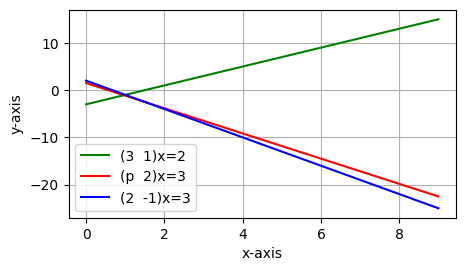
\includegraphics[width=\columnwidth]{chapters/11/10/4/9/fig/11.10.4.9.png}
    \caption{}
    \label{11.10.4.9}
\end{figure}
